\documentclass[signature=data]{physicsreport}

%%
%% User settings
%%

\classno{}
\stuno{}
\groupno{}
\stuname{}
\expdate{\expdatefmt\today}
\expname{迈克尔逊干涉仪实验}

%%
%% Document body
%%

\begin{document}
% First page
% Some titles and personal information are defined in ``\maketitle''.
\maketitle

\section{预习}
\begin{enumerate}
    \item 结合下图迈克尔逊干涉仪的等效光路图,推导出光程差的表达式$\Delta L = 2hcos\alpha$。
    \begin{figure}[htbp]
    \flushright
    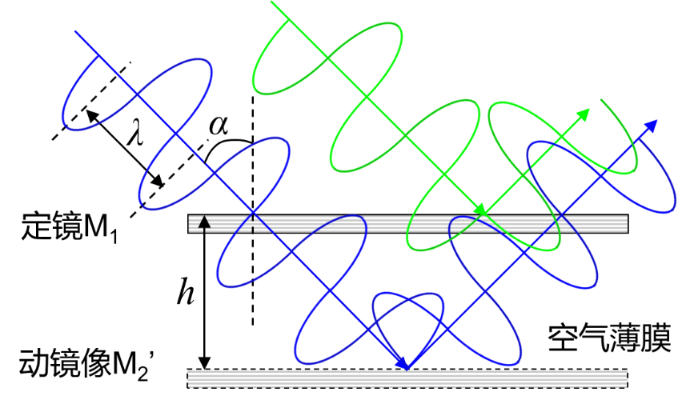
\includegraphics{images/lab1/figure1.png}
    \end{figure} 
    \vspace{3cm}
    \item 本实验将测量He-Ne激光的波长$\lambda$,若等倾干涉圆环每变化50环,动镜$M_2$对应的螺旋测微器读数变化为$d$(注意:$M_2$实际移动距离为$d/20$),根据光程差的表达式光程差$\Delta L = 2hcos\alpha$,结合中心圆环对应的倾角$\alpha \approx 0$这一近似条件,推导出波长$\lambda$的表达式(提示:光程差每改变1个波长,干涉圆环变化1环)。
    \vspace{5cm}
\end{enumerate}

% Teacher signature
\makeatletter
\physicsreport@body@signature{preparation}
\makeatother

\section{实验目的及任务}
\begin{enumerate}
    \item 了解迈克尔孙干涉仪的结构、原理及调节方法;
    \item 观察光的非定域和定域干涉现象,包括等倾和等厚干涉;
    \item 逐差法测定He-Ne激光波长;
    \item 作图法计算空气的折射率。
\end{enumerate}
\vspace{0.7cm}
% Original experiment data
\section{原始数据记录}
\subsection{}
\begin{table}[H]
    \caption{测定 He-Ne 激光波长数据} \label{tab:1}
    \centering
    \begin{tabularx}{\textwidth}{|c|Y|Y|Y|Y|Y|Y|} \hline
        圆环变化数目          & 0 & 50 & 100 & 150 & 200 & 250 \\\hline
        $M_2$ 位置读数 (mm) &   &    &     &     &     &     \\\hline
    \end{tabularx}
\end{table}

\subsection{}
\begin{table}[H]
    \caption{测定空气折射率数据} \label{tab:2}
    \centering
    \begin{tabularx}{\textwidth}{|c|Y|Y|Y|Y|Y|} \hline
        气室内压强 (mmHg) & 50 & 100 & 150 & 200 & 250 \\\hline
        干涉条纹变化数      &    &     &     &     &     \\\hline
        干涉条纹变化数      &    &     &     &     &     \\\hline
        干涉条纹变化数      &    &     &     &     &     \\\hline
    \end{tabularx}
\end{table}

\subsection{观察等倾和等厚现象, 并附现象图.}

% Teacher signature
\makeatletter
\physicsreport@body@signature{data}
\makeatother

\newpage
% Data process and others
\section{数据处理}
\begin{enumerate}
    \item 利用逐差法计算 He-Ne 激光波长.
    
    由预习可知,若已知变化了$k$个环时,测微器变化距离为$d$,可根据下式求出波长:
    $$
    k\lambda=2*\frac{d}{20}=\frac{d}{10}
    $$
    利用逐差法代入数据计算可得
    $$
    \Bar{\lambda}=\frac{\sum\limits_{i=1}^3{d_{i+3}-d_{i}}}{3*10*150}=650nm
    $$
    \item 作出条纹变化数 $\Delta n$ 相对于气压变化 $\Delta p$ 的曲线, 用图解法计算斜率, 求出空气的折射率.
    \begin{figure}[htbp]
    \centering
    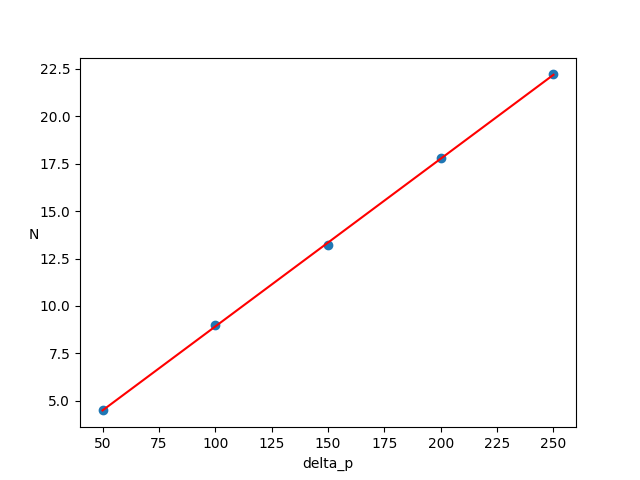
\includegraphics[width=0.7\linewidth]{images/lab1/p-N.png}
    \end{figure} 
    
    先利用最小二乘法计算近似直线,再通过计算出的斜率通过公式计算出出空气的折射率
    $$\hat{a}=0.0884,\hat{b}=0.08$$
    $$n=1+\frac{\bar{\lambda} P_{a m b}}{2 l} \frac{N}{\Delta p}=1.0025$$
    \item 记录等倾和等厚现象, 特点并分析.

    \begin{figure}[H]
	\centering
	\begin{minipage}{0.39\linewidth}
		\centering
		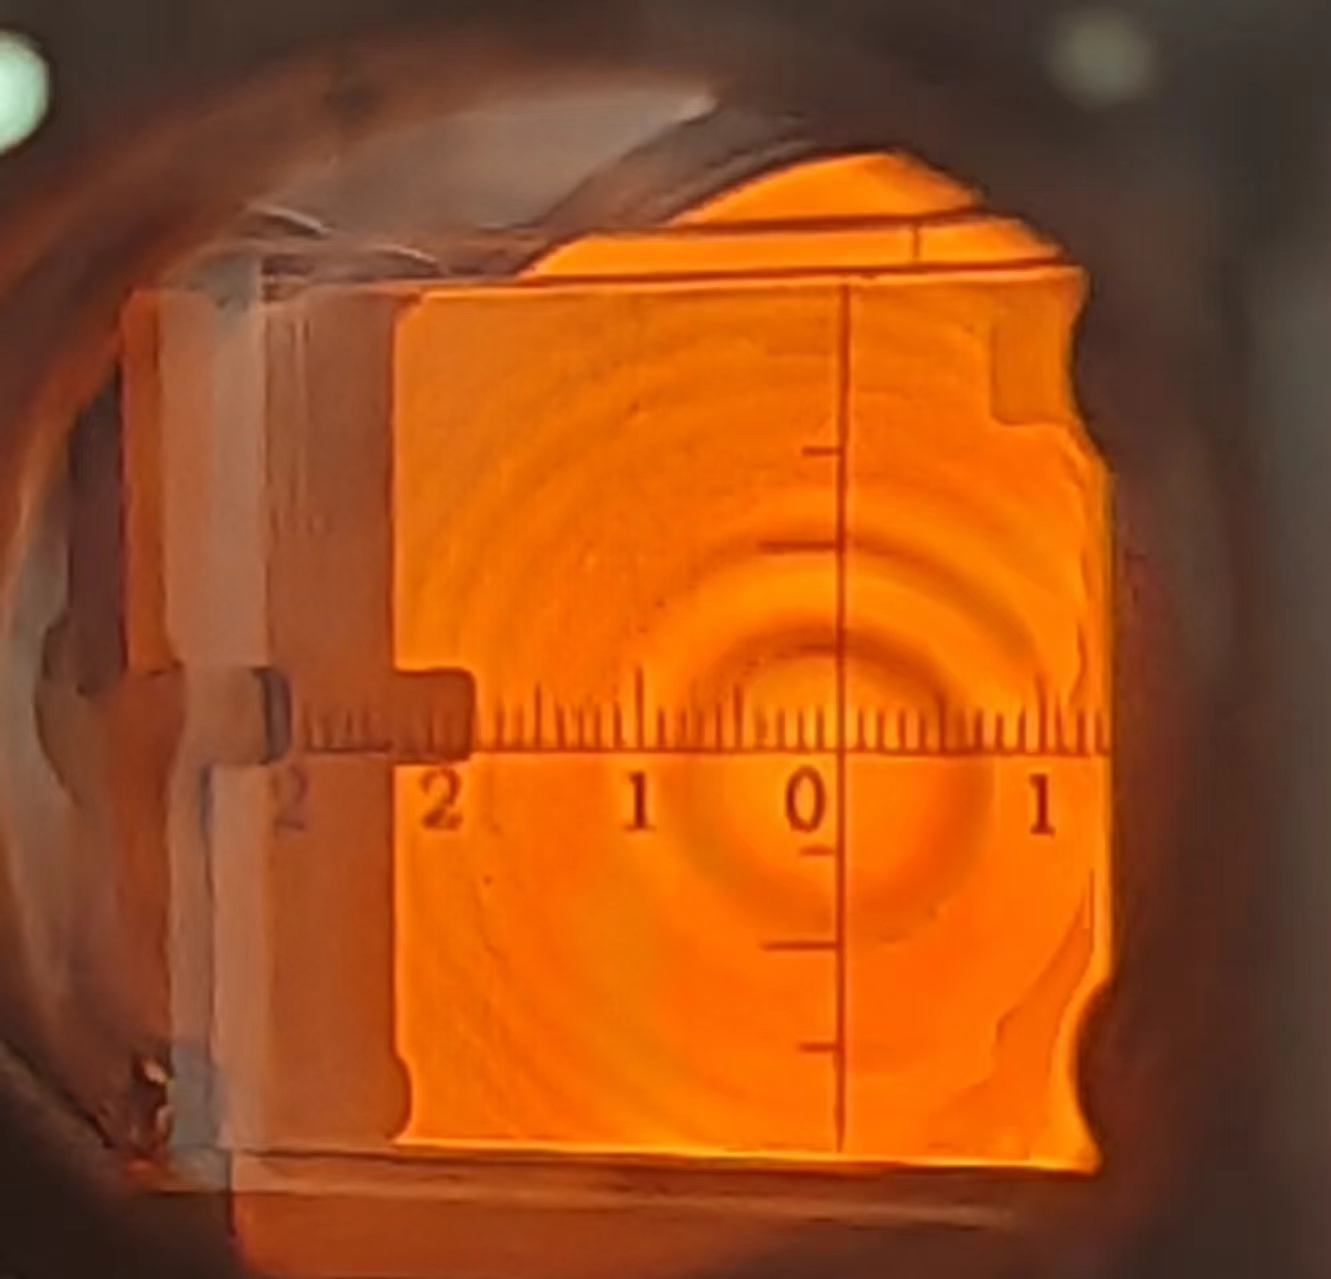
\includegraphics[width=0.9\linewidth]{images/lab1/等倾.jpg}
		\caption{等倾}
		\label{chutian1}%文中引用该图片代号
	\end{minipage}
	\begin{minipage}{0.35\linewidth}
		\centering
		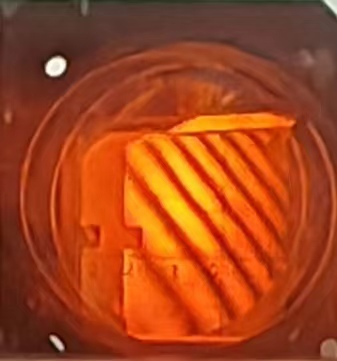
\includegraphics[width=0.9\linewidth]{images/lab1/等厚.jpg}
		\caption{等厚}
		\label{chutian2}%文中引用该图片代号
	\end{minipage}
    \end{figure}

 \hspace{2em}
    等倾条纹的特点是同心圆环,中间较疏,越向外越密。这正是因为同一特定光程差的干涉发生在某距成像中心的特定距离。

     \hspace{2em}
    等厚条纹的特点是平行明暗条纹。当定镜、动镜像夹角很小时,可视作其间存在一线性空气薄层,可以发生等厚干涉。

     \hspace{2em}
通过仔细调节,我们可以成功将动镜反射中心的像成在定镜反射中心处,从而获得比较标准的直平行等厚条纹。

\end{enumerate}


\section{讨论题}
\begin{enumerate}
    \item 归纳非定域干涉和定域干涉的特点.
    
    \hspace{2em}
      对于相干性较差的光源,在调整光路得到干涉条纹的过程中,只能在较小的调节范围内看到清晰的干涉条纹,即定域干涉。这时需要缓慢地调节出对应的图样。

     \hspace{2em}
   对于相干性较好的光源,在调整光路得到干涉条纹的过程中,可以在较大的调节范围内看到清晰的干涉条纹,即非定域干涉。往往不用特意调节就可以产生干涉条纹。
    \item 迈克尔逊干涉仪所产生的干涉条纹疏密程度是由什么因素决定的? 变化规律怎样?

     \hspace{2em}
     干涉条纹变化的本质原因就是光程差发生了变化。某点干涉条纹变密是因为该点附近光程差变化的速度变快了。也因为这个原理,当压力气室气压增大时,折射率会增大,条纹因此会变密。同时改变动镜,定镜的角度和高度也会导致条纹疏密发生变化。因为光路全体发生了变化,因此对应点的光程差发生了变化,条纹疏密也很大可能会发生变化。
    \item 说明仪器要设计补偿片的原因.

     \hspace{2em}
    在半透半反镜和动镜之间设置的补偿板是与半透半反镜厚度相同,方向平行的。这个补偿板是为了保证透射光和反射光的光程相同。如果没有补偿板,会导致两束光差了两个半透半反镜对应的光程。为了抵消这个误差,所以设计了一个补偿片。
\end{enumerate}

\end{document}